\documentclass{beamer}
\usetheme{metropolis}
\setbeamercolor{background canvas}{bg=white}
\usepackage{graphicx}
\graphicspath{{../dissertation/graphics/}}
\usepackage{natbib}
\usepackage{lmodern}
\usepackage[most]{tcolorbox}
\usepackage{tabularx}
\usepackage{colortbl} 
\newcolumntype{Y}{>{\centering\arraybackslash}X}
\newtcolorbox[blend into=tables]{colortable}[2][]{
	colback=white,
	tabularx*={\renewcommand{\arraystretch}{1.0}}{Y|Y|Y|Y|Y|Y},title={#2},boxrule=0.8pt, center title
}

\title{Hyper Heuristic Cryptography with Mixed Adversarial Nets}
\date{\today}
\author{\textbf{Author:} Aly Shmahell \\ \textbf{Supervisor:} Prof. Giovanni De Gasperis}
\institute{University of L'Aquila}
\begin{document}
	\maketitle
	\section{Introduction}
		\begin{frame}{What This Thesis Is About}
			\vfill
			\textbf{Neural Cryptography:} \\
			{\centering
				applying stochastic methods to get neural nets to achieve cryptographic functionality.
				\par}
			\vfill
			\textbf{Basis For This Thesis:}\\
			{\centering
				a recent paper released in 2016 from Google Brain~\citep{DBLP:journals/corr/AbadiA16}.
				\par}
			\vfill
			\textbf{How The Thesis Extends Its Basis:}\\
			{\centering
				by focusing on increasing confidentiality of communication, while minimizing loss of information integrity.
			\par}
		\end{frame}
		\begin{frame}{Basic Cryptology Scheme}
			\begin{center}
				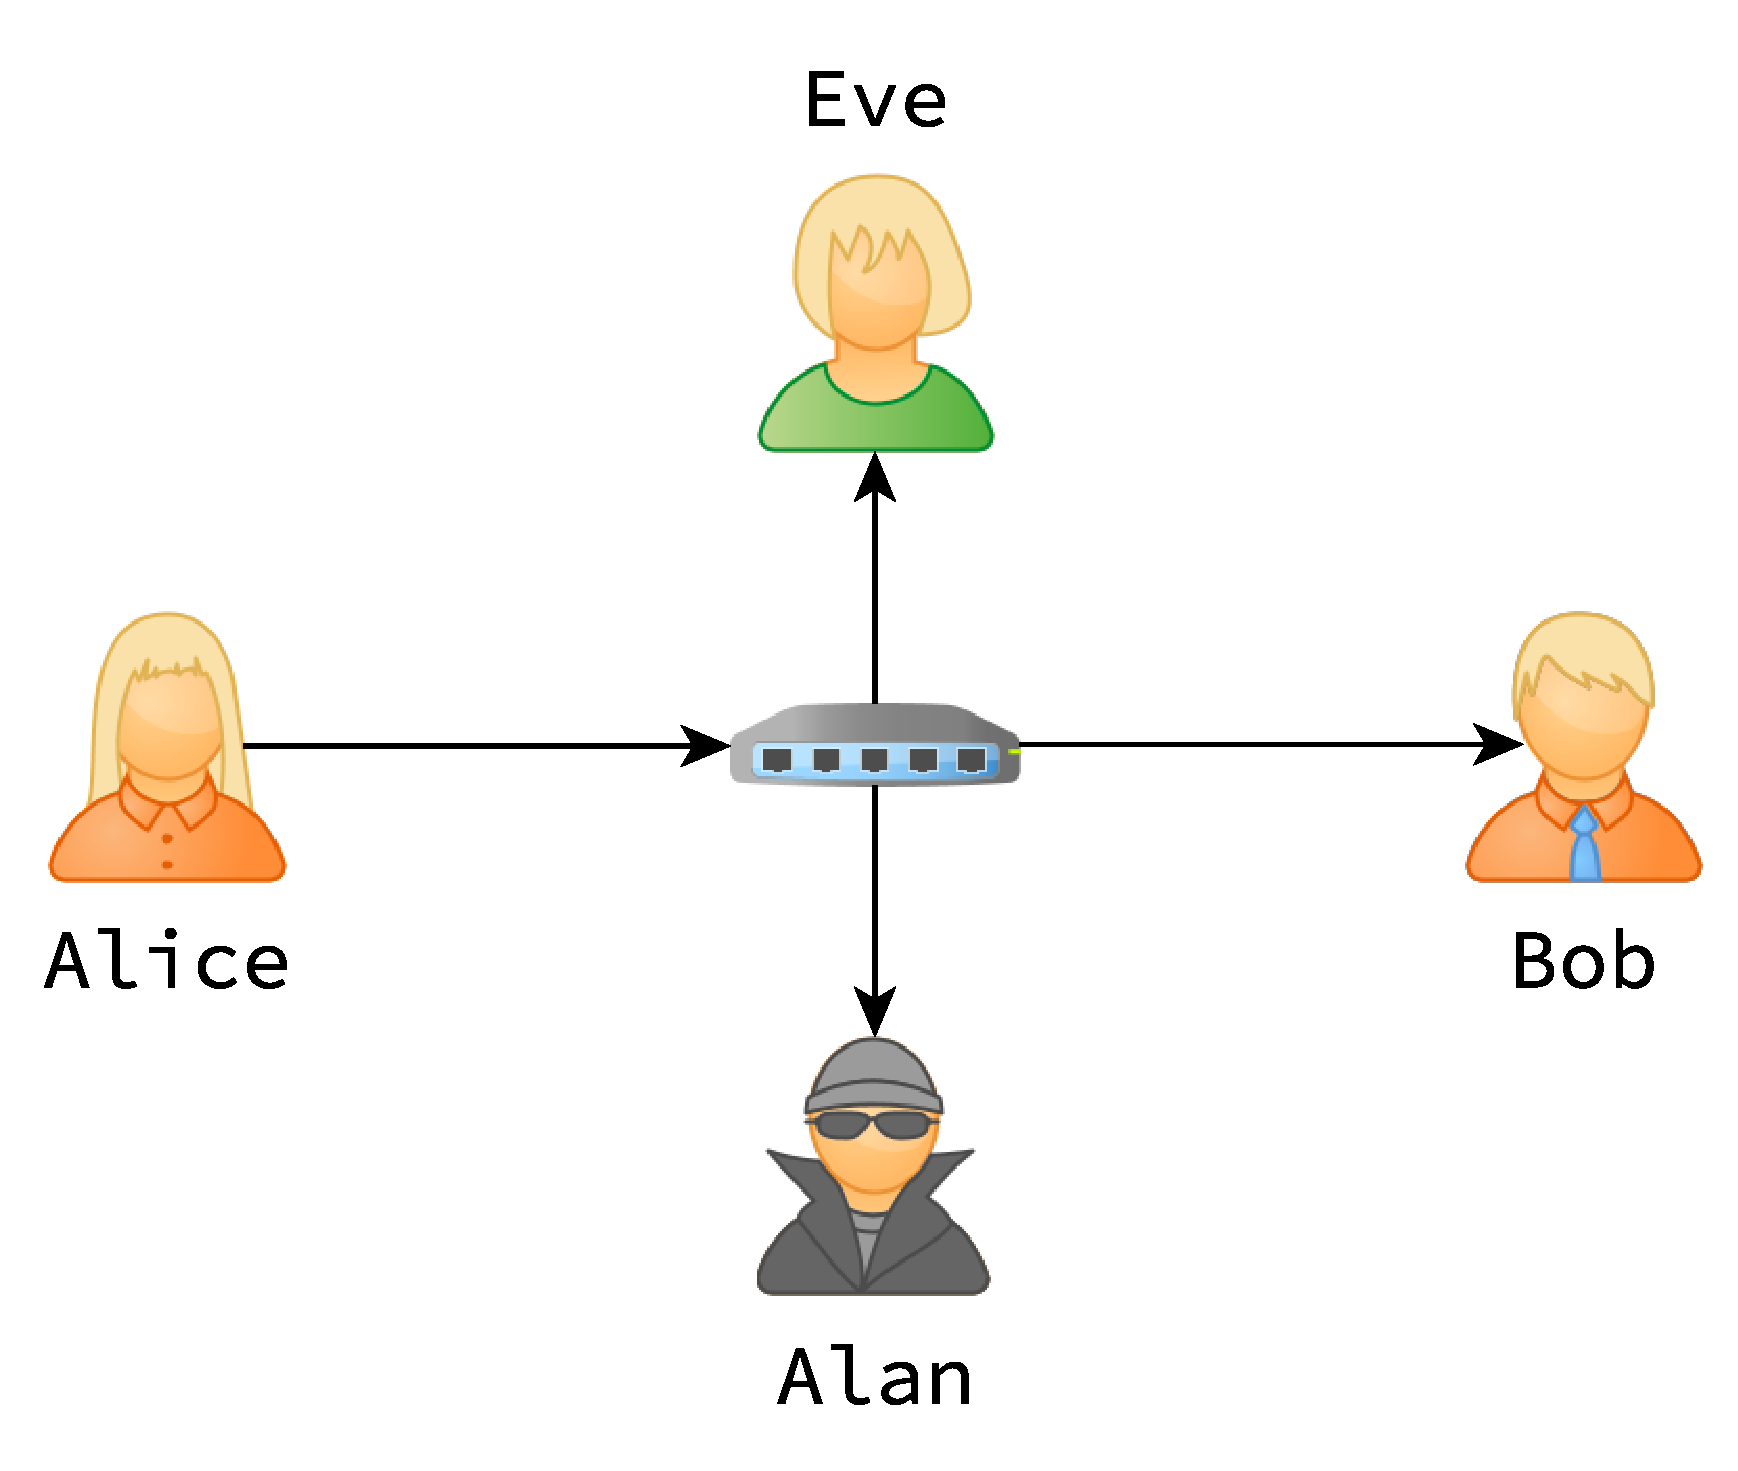
\includegraphics[height=0.8\textheight]{Alice-Bob-Eve-Alan}
			\end{center}
		\end{frame}
		\begin{frame}{Symmetric Results From Google Brain - For Comparison}
			\begin{center}
				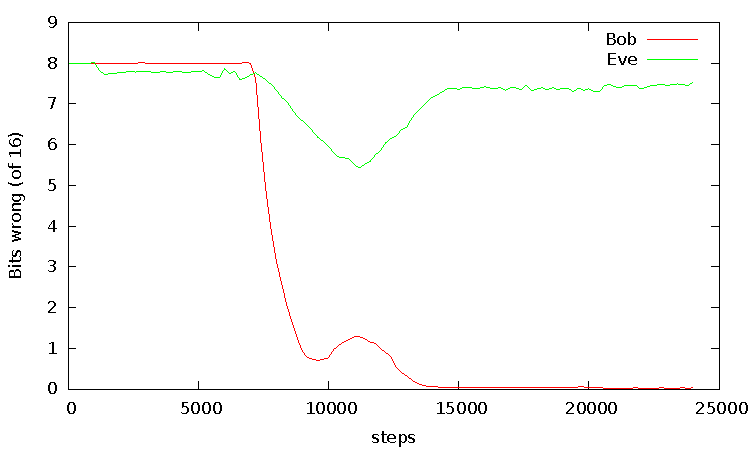
\includegraphics[height=0.8\textheight]{cryptolearn_batch_tighter}
			\end{center}
		\end{frame}
		\begin{frame}{Asymmetric Results From Google Brain - For Comparison}
			\begin{center}
				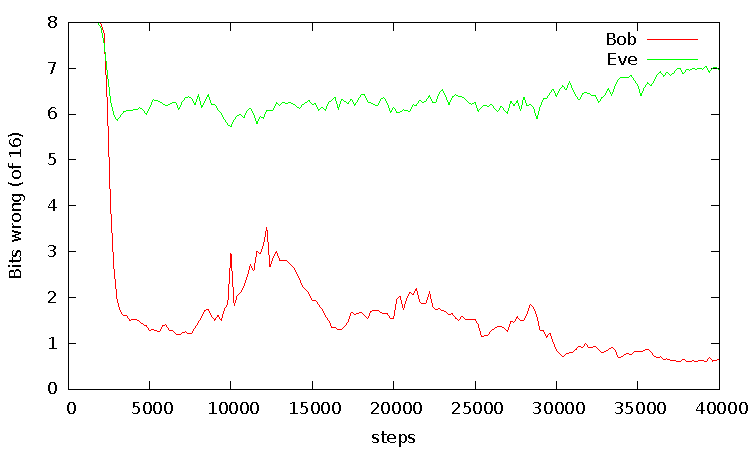
\includegraphics[height=0.8\textheight]{pubkey_bob_v_eve}
			\end{center}
		\end{frame}
		\begin{frame}{Justification For Neural Cryptography}
			 \vfill
			 \textbf{Neural Cryptography Is Viable:}\\
			 {\centering
			 	convolutional nets can construct local spatial relations in data.
			 	\par}
			 \vfill
			 \textbf{Neural Cryptanalysis Is Viable:}\\
			 {\centering
			 	fully connected layers can detect global spatial relations in data.
			 	\par}
			 \vfill
			 \textbf{Neural Cryptography Can Be Fast:}\\
			 {\centering
			 	convolutional nets share weights using their filters.
			 	\par}
			 \vfill
			 \textbf{Neural Cryptography Is Evolved, Not Patched:}\\
			 {\centering
			 	using adversary in training evolves weights which serves to tweak the cryptographic functionality.
			 	\par}
		\end{frame}
		\begin{frame}{What This Thesis Adds To The Research Pool}
			\vfill
			\textbf{A Prototype Blueprint:}\\
			{\centering
				for a software-engineered neural crypto-system.
				\par}
			\vfill
			\textbf{An Analysis Of How Neural Components Work:}\\
			{\centering
				when the objective is to achieve cryptographic functionality.
				\par}
			\vfill
			\textbf{An Enhancement In The Neural Structures:}\\
			{\centering
				which yields a boost in cryptographic robustness.
			\par}
			\vfill
			\textbf{Transfer Learning:}\\
			{\centering
				to get symmetric neural cryptography on par with asymmetric neural cryptography.
			\par}
		\end{frame}
		\section{Experiments \& Results}
		\begin{frame}{Symmetric Scheme}
			\begin{center}
				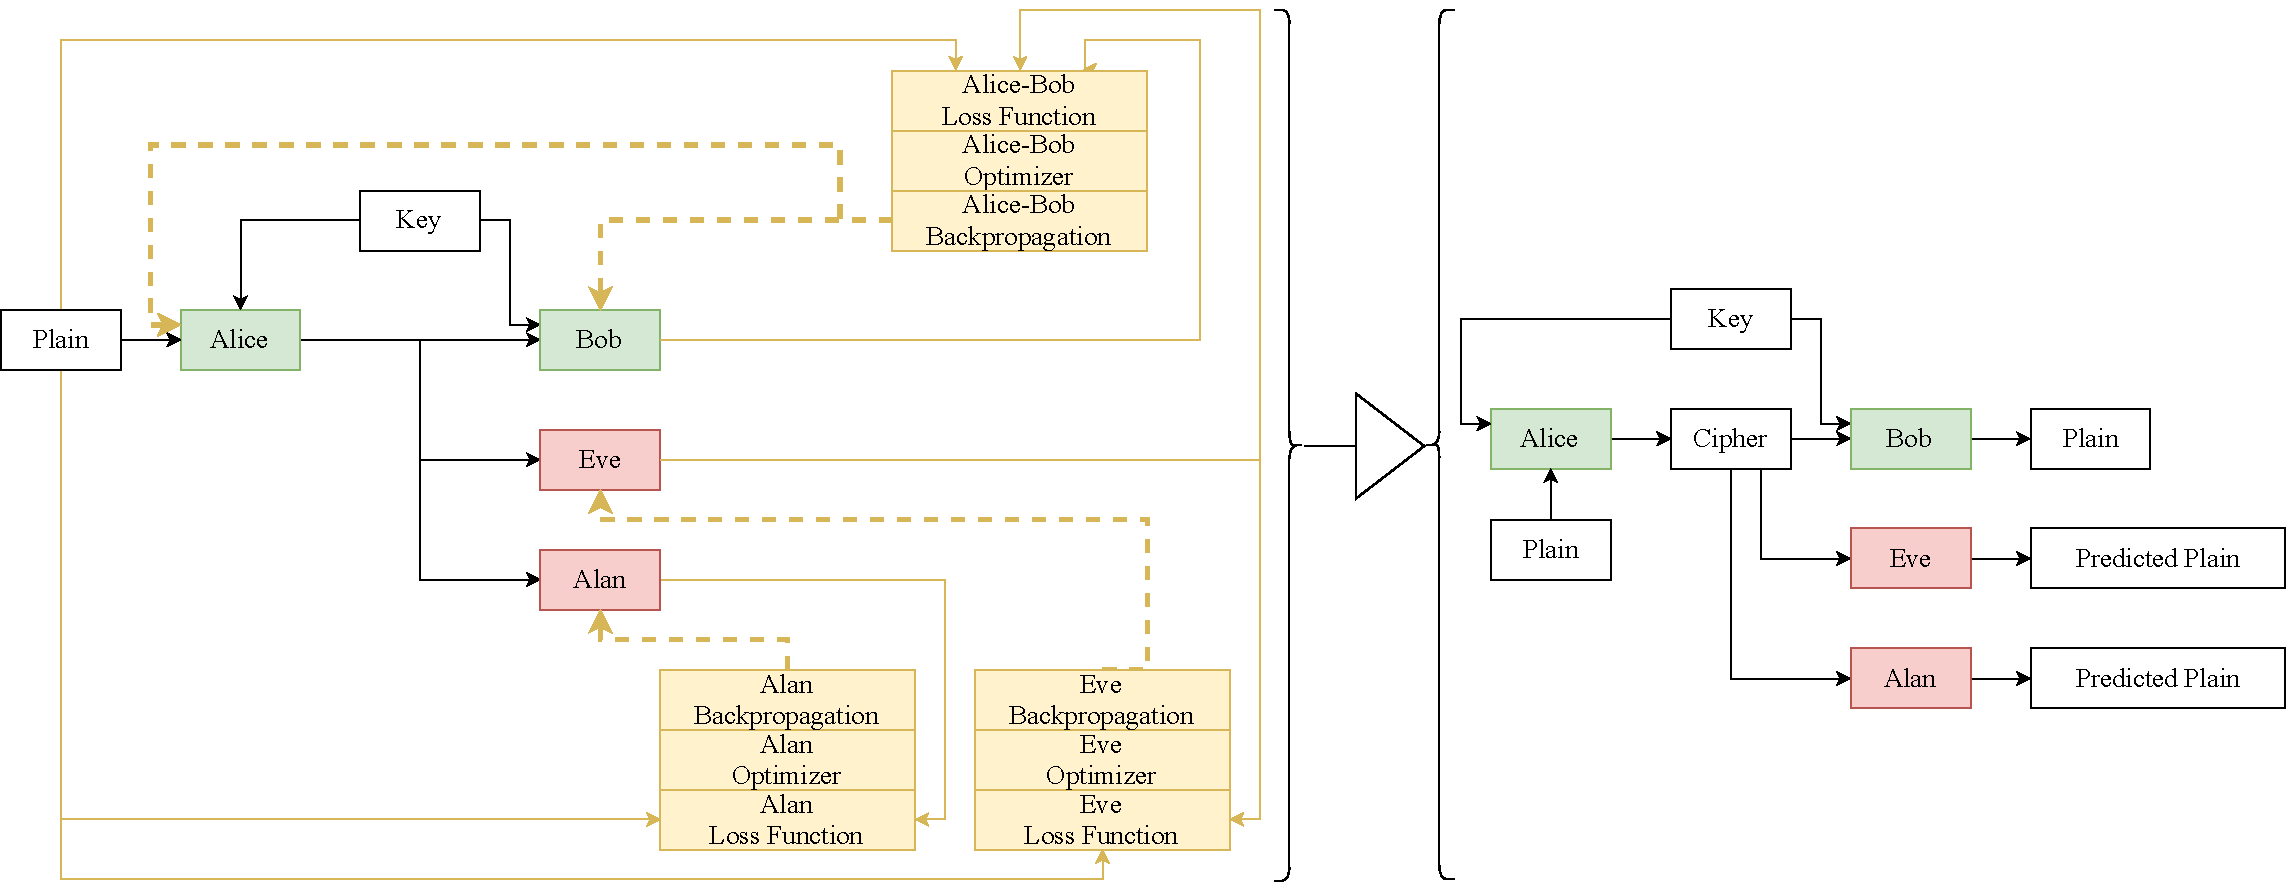
\includegraphics[width=\textwidth, height=0.8\textheight]{symmetricScheme-present}
			\end{center}
		\end{frame}
		\begin{frame}{Thesis Results - Symmetric Training}
			\begin{center}
				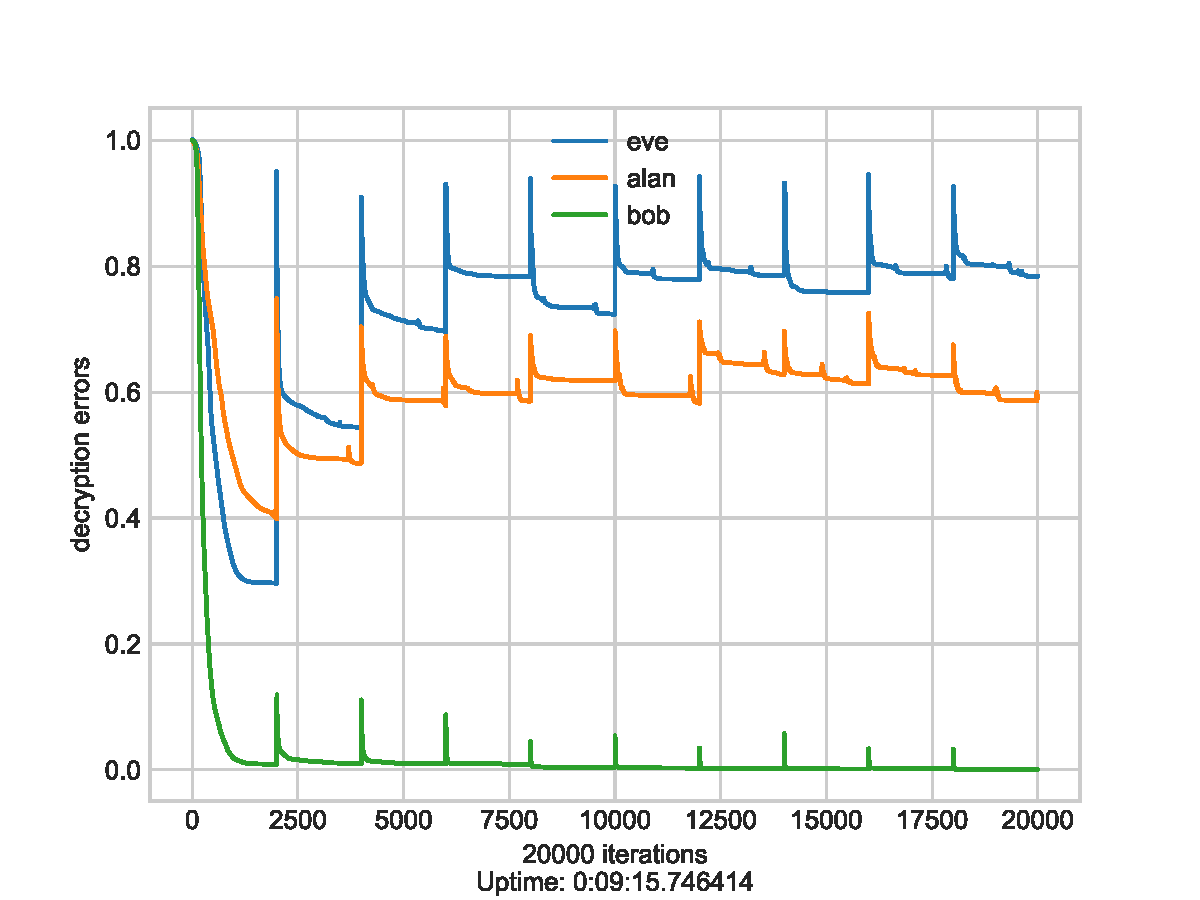
\includegraphics[height=0.9\textheight]{neurencoder-symmetric-training}
			\end{center}
		\end{frame}
		\begin{frame}{Thesis Results - Symmetric Testing}
			\begin{center}
				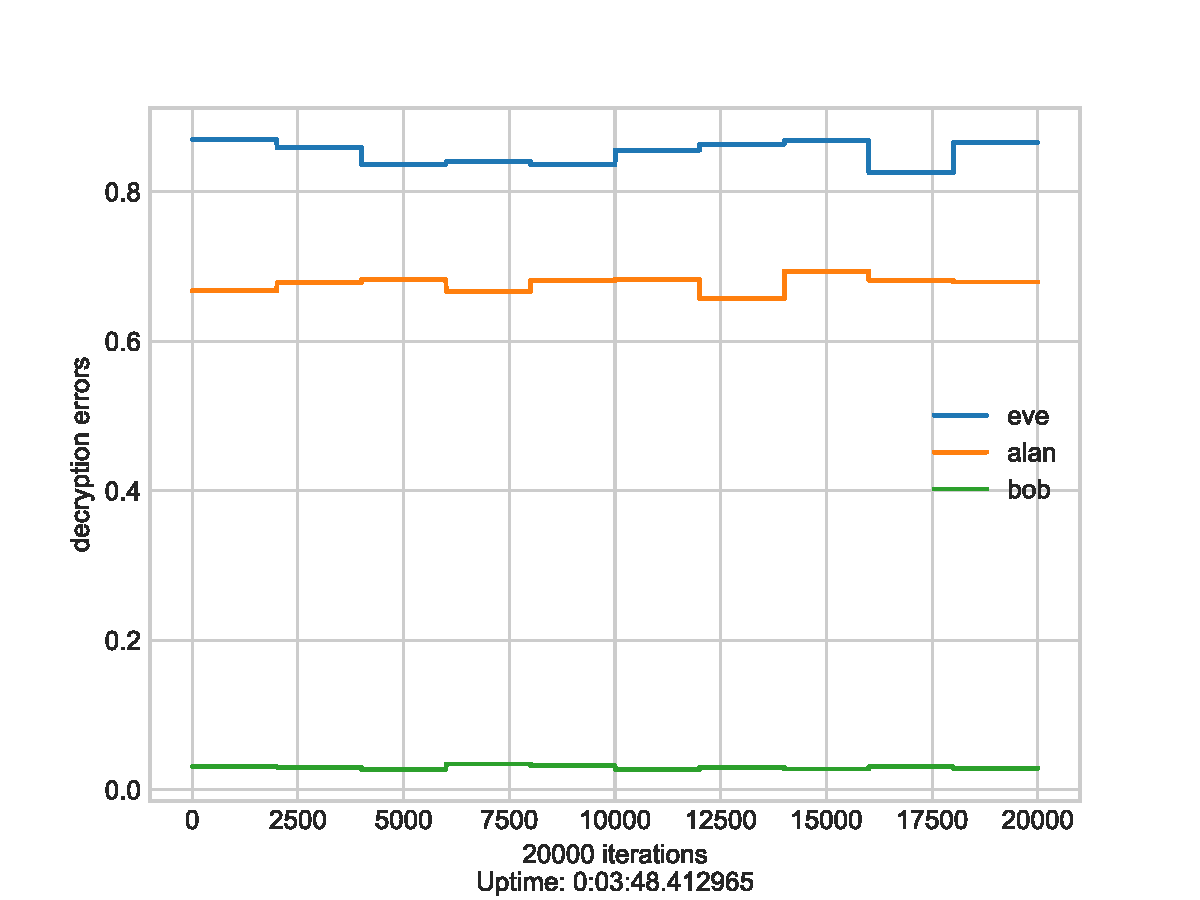
\includegraphics[height=0.9\textheight]{neurencoder-symmetric-testing}
			\end{center}
		\end{frame}
		\begin{frame}{Asymmetric Scheme}
			\begin{center}
				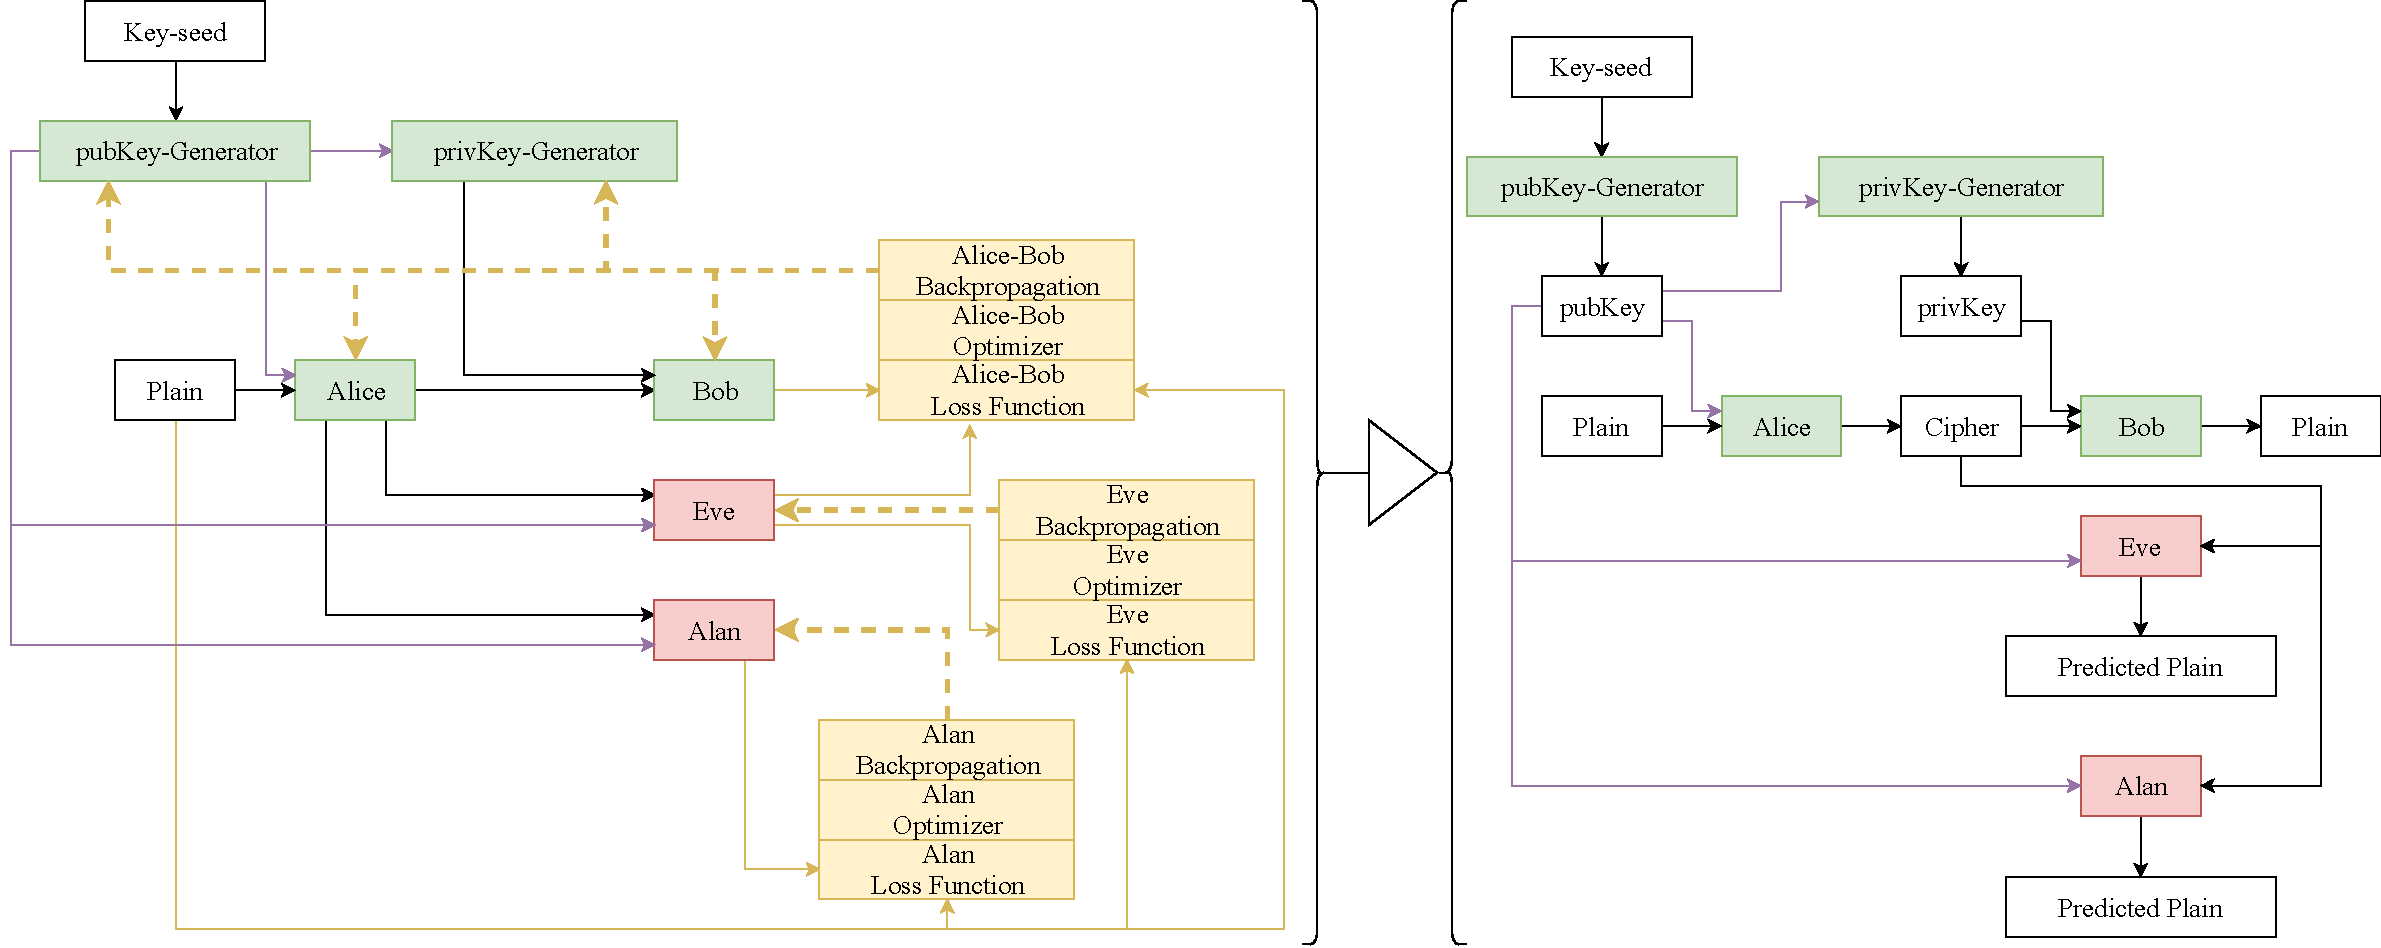
\includegraphics[width=\textwidth, height=0.8\textheight]{asymmtericScheme-present}
			\end{center}
		\end{frame}
		\begin{frame}{Thesis Results - Asymmetric Training}
			\begin{center}
				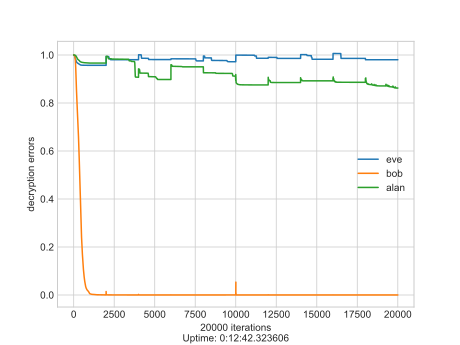
\includegraphics[height=0.9\textheight]{neurencoder-asymmetric-training}
			\end{center}
		\end{frame}
		\begin{frame}{Thesis Results - Asymmetric Testing}
			\begin{center}
				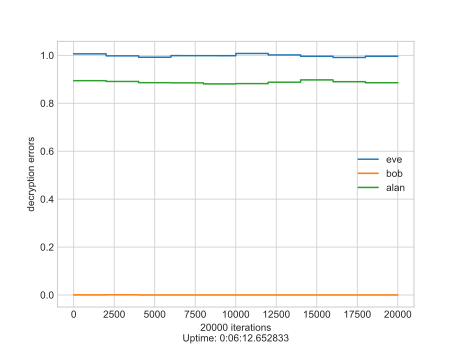
\includegraphics[height=0.9\textheight]{neurencoder-asymmetric-testing}
			\end{center}
		\end{frame}
		\begin{frame}{Transfer Learning}
			\textbf{Transfer Learning:}\\
			{\centering
				Given a source domain $ D_{S} $ and learning task $ T_{S} $ , a target domain $ D_{T} $ and learning task
				$ T_{T} $ , transfer learning aims to help improve the learning of the
				target predictive function $ f_{T}(\cdot) $ in $ D_{T} $ using the knowledge in
				$ D_{S} $ and $ T_{S} $ , where $ D_{S} \neq D_{T} $ , or $ T_{S} \neq T_{T} $.~\citep{5288526}
				\par} 
		\end{frame}
		\begin{frame}{Hybrid Scheme}
			\begin{center}
				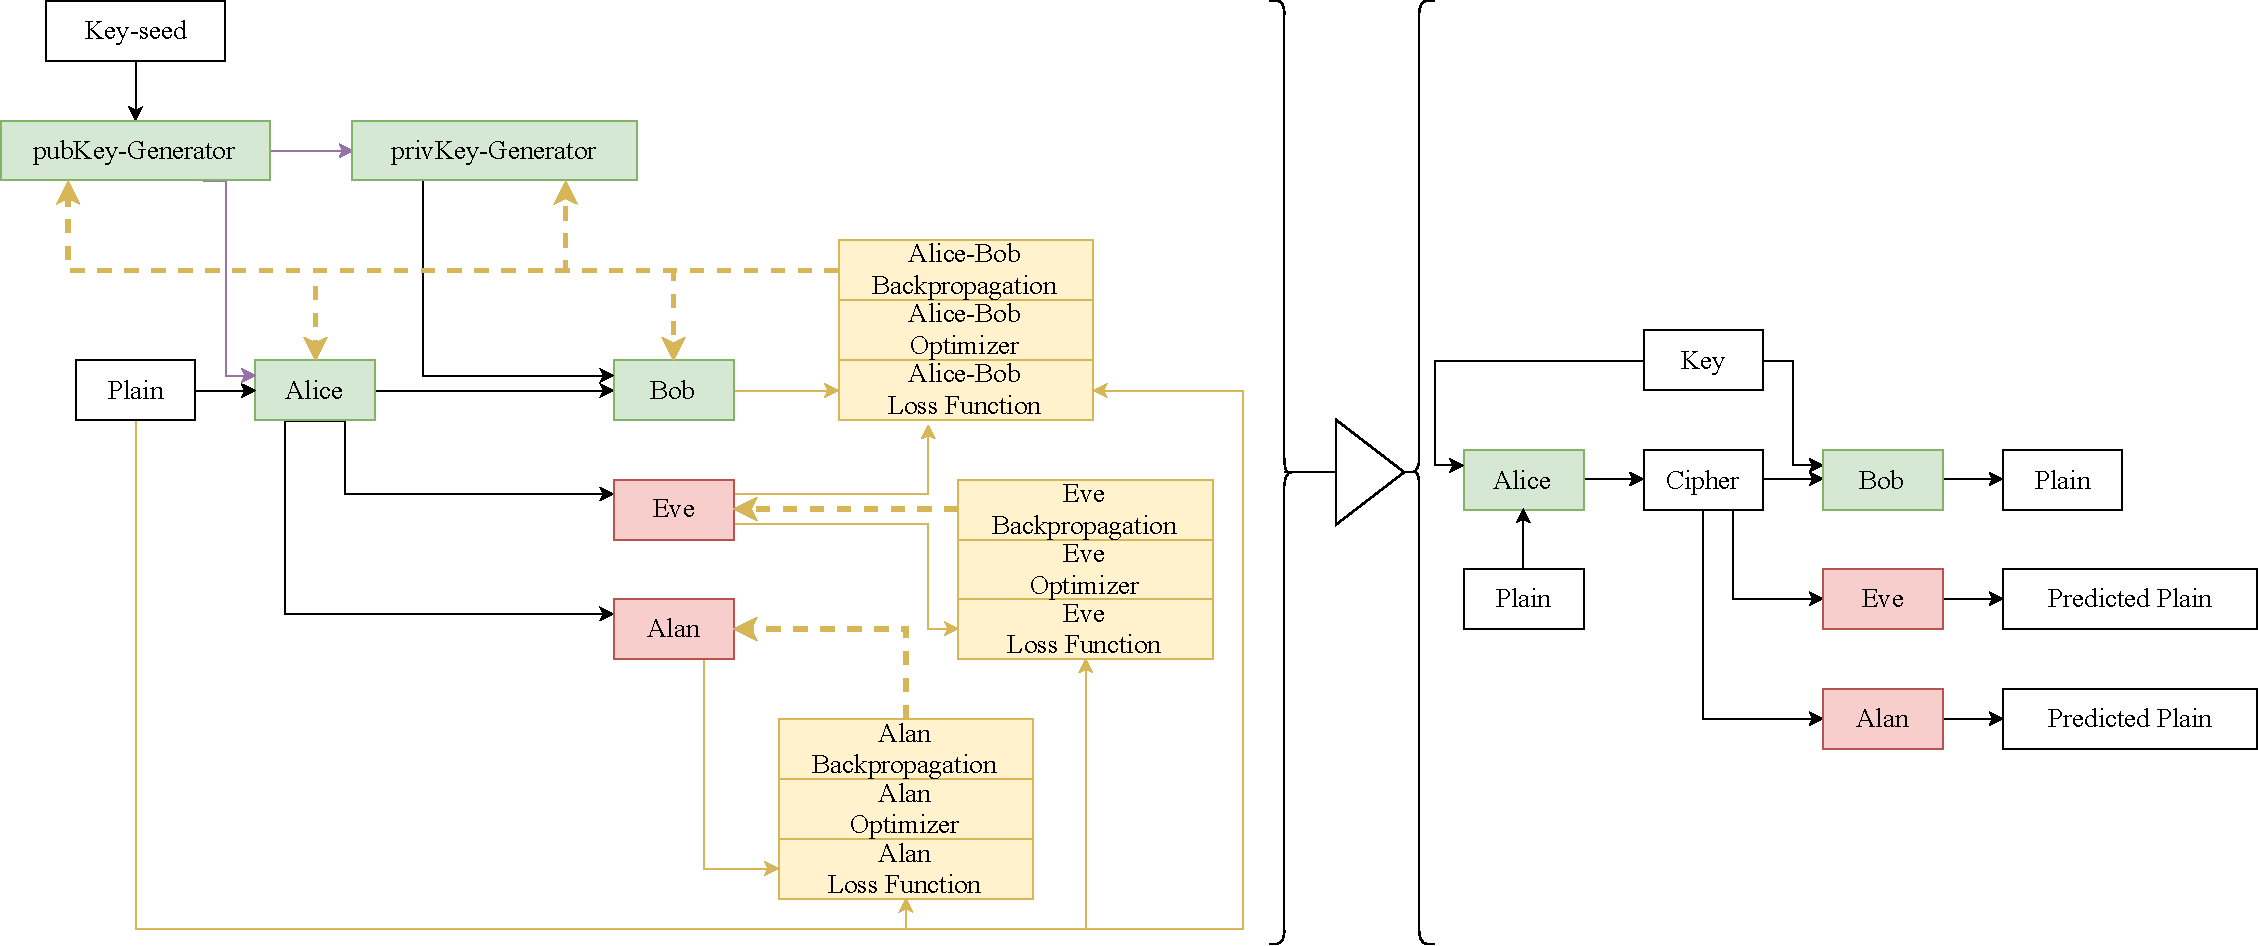
\includegraphics[width=\textwidth, height=0.8\textheight]{hybridScheme-present}
			\end{center}
		\end{frame}
		\begin{frame}{Thesis Results - Hybrid Training}
			\begin{center}
				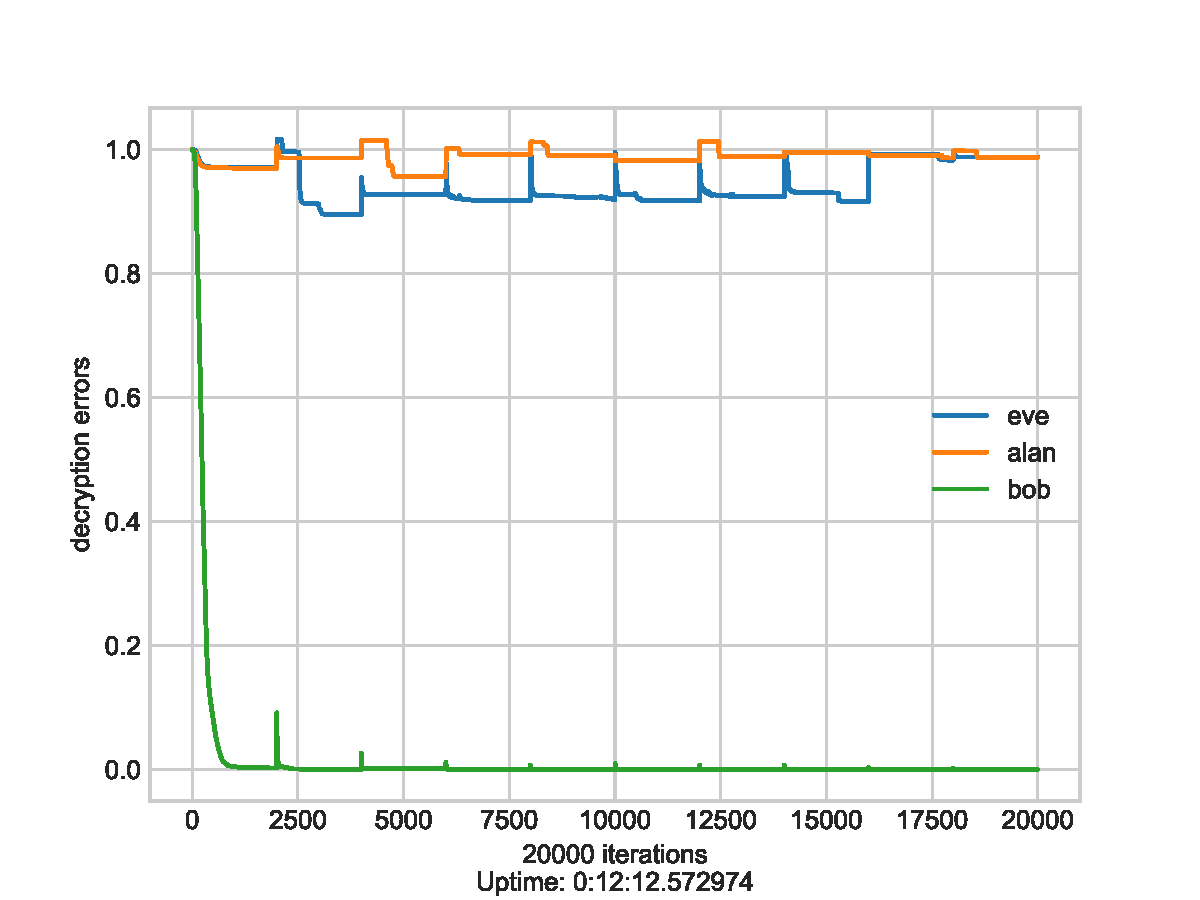
\includegraphics[height=0.9\textheight]{neurencoder-hybrid-training}
			\end{center}
		\end{frame}
		\begin{frame}{Thesis Results - Hybrid Testing}
			\begin{center}
				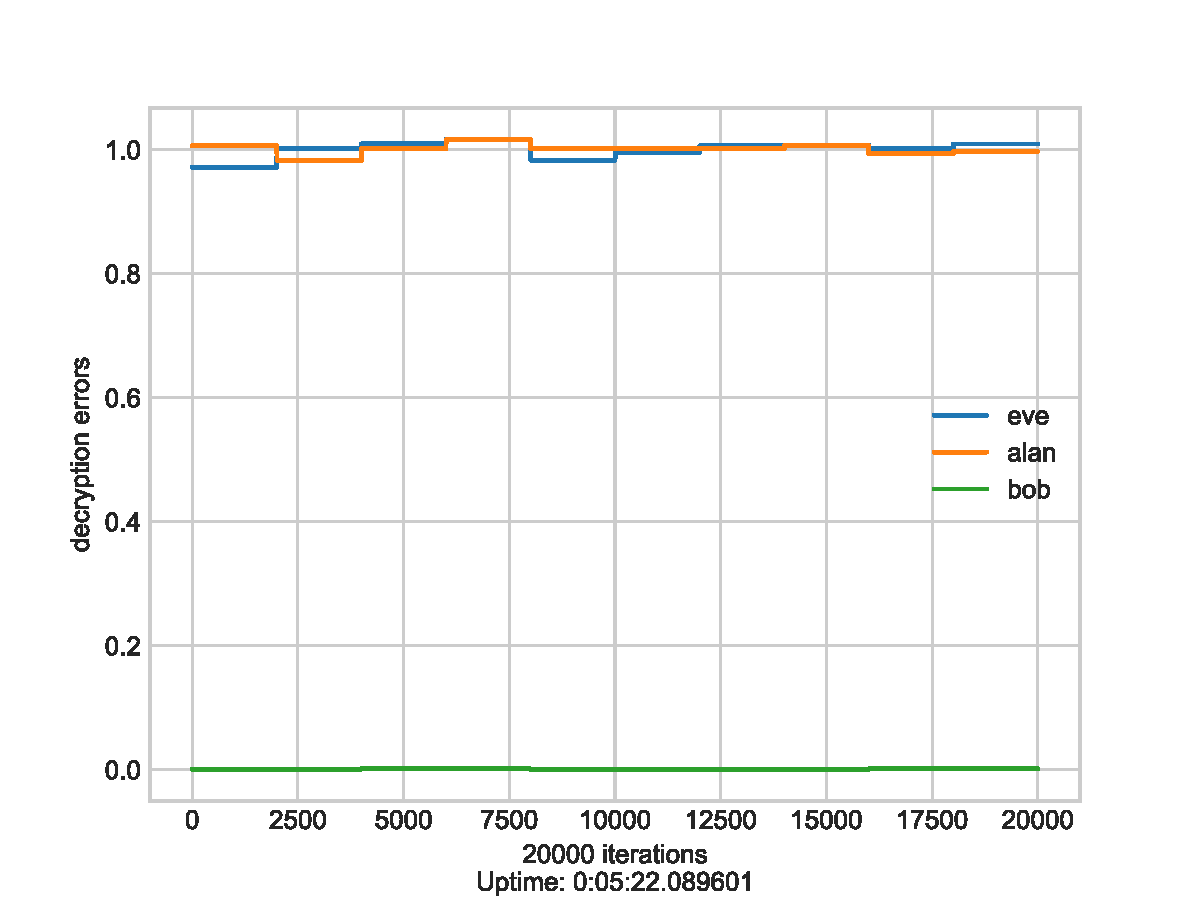
\includegraphics[height=0.9\textheight]{neurencoder-hybrid-testing}
			\end{center}
		\end{frame}	
		\section{Implementation}
		\begin{frame}{Class Diagram}
			\begin{center}
				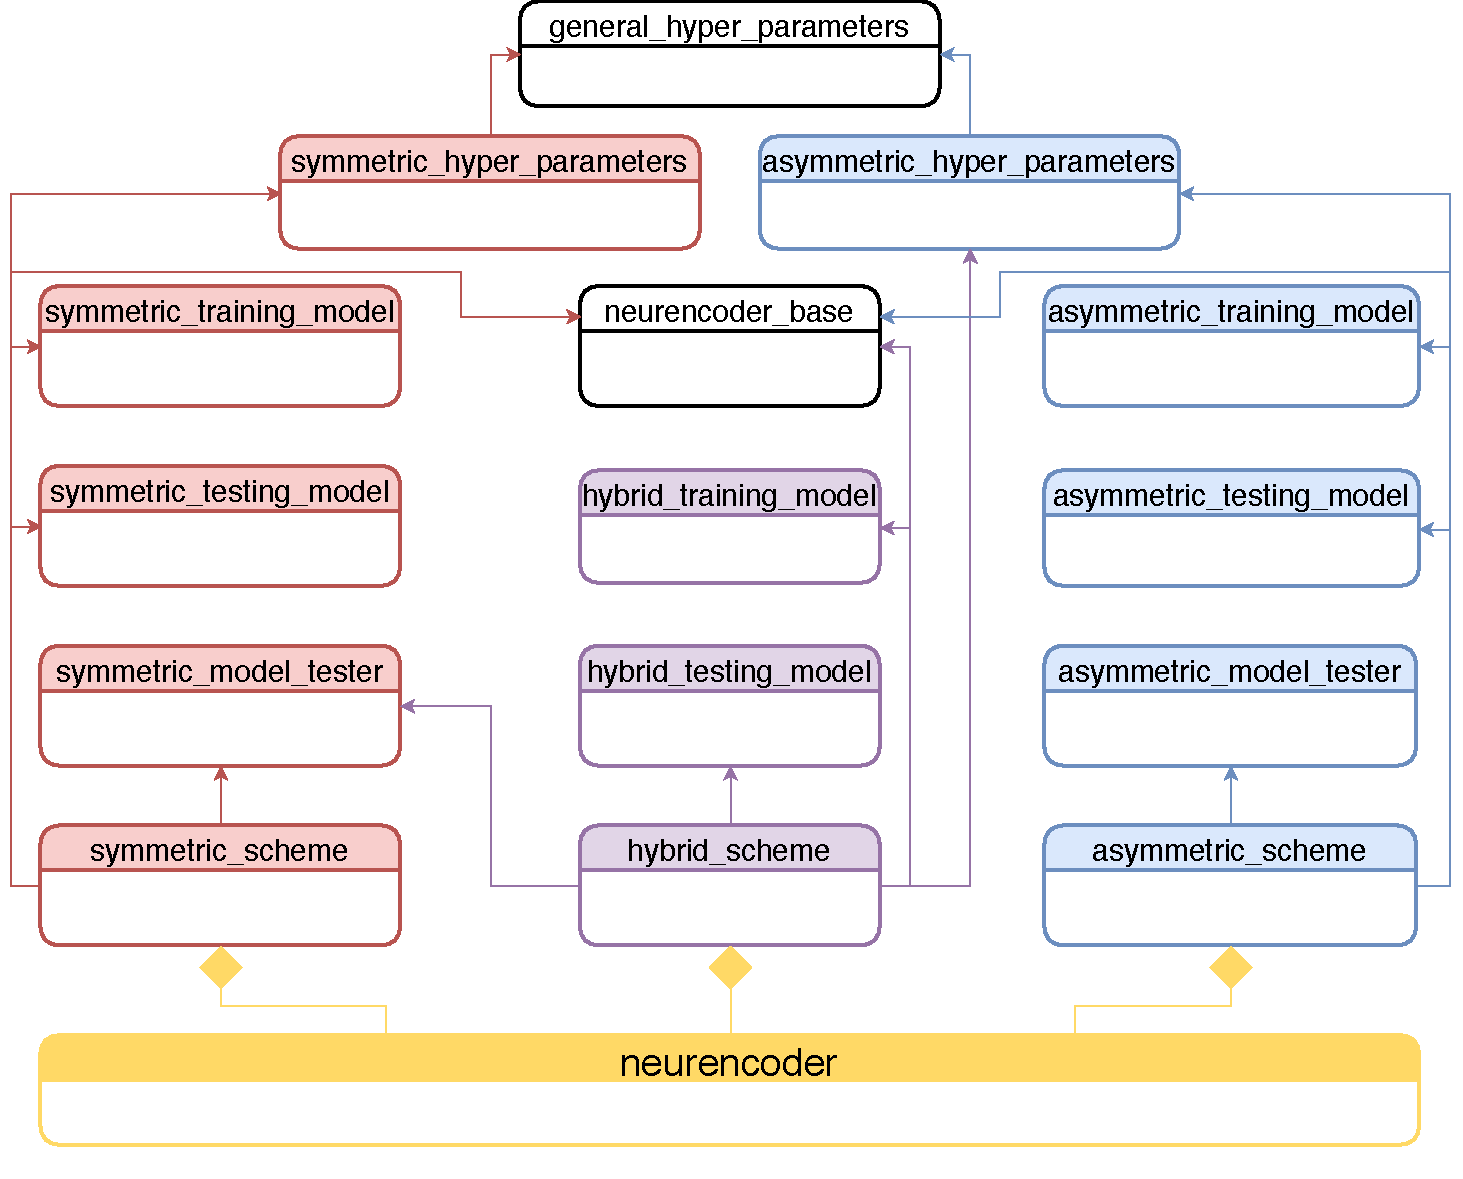
\includegraphics[height=0.9\textheight]{classDiagram-present}
			\end{center}
		\end{frame}	
	\section{Appendix:{\tiny } How I Chose My Activation Functions}
	\begin{frame}{Dummy Net Example}
		\begin{center}
			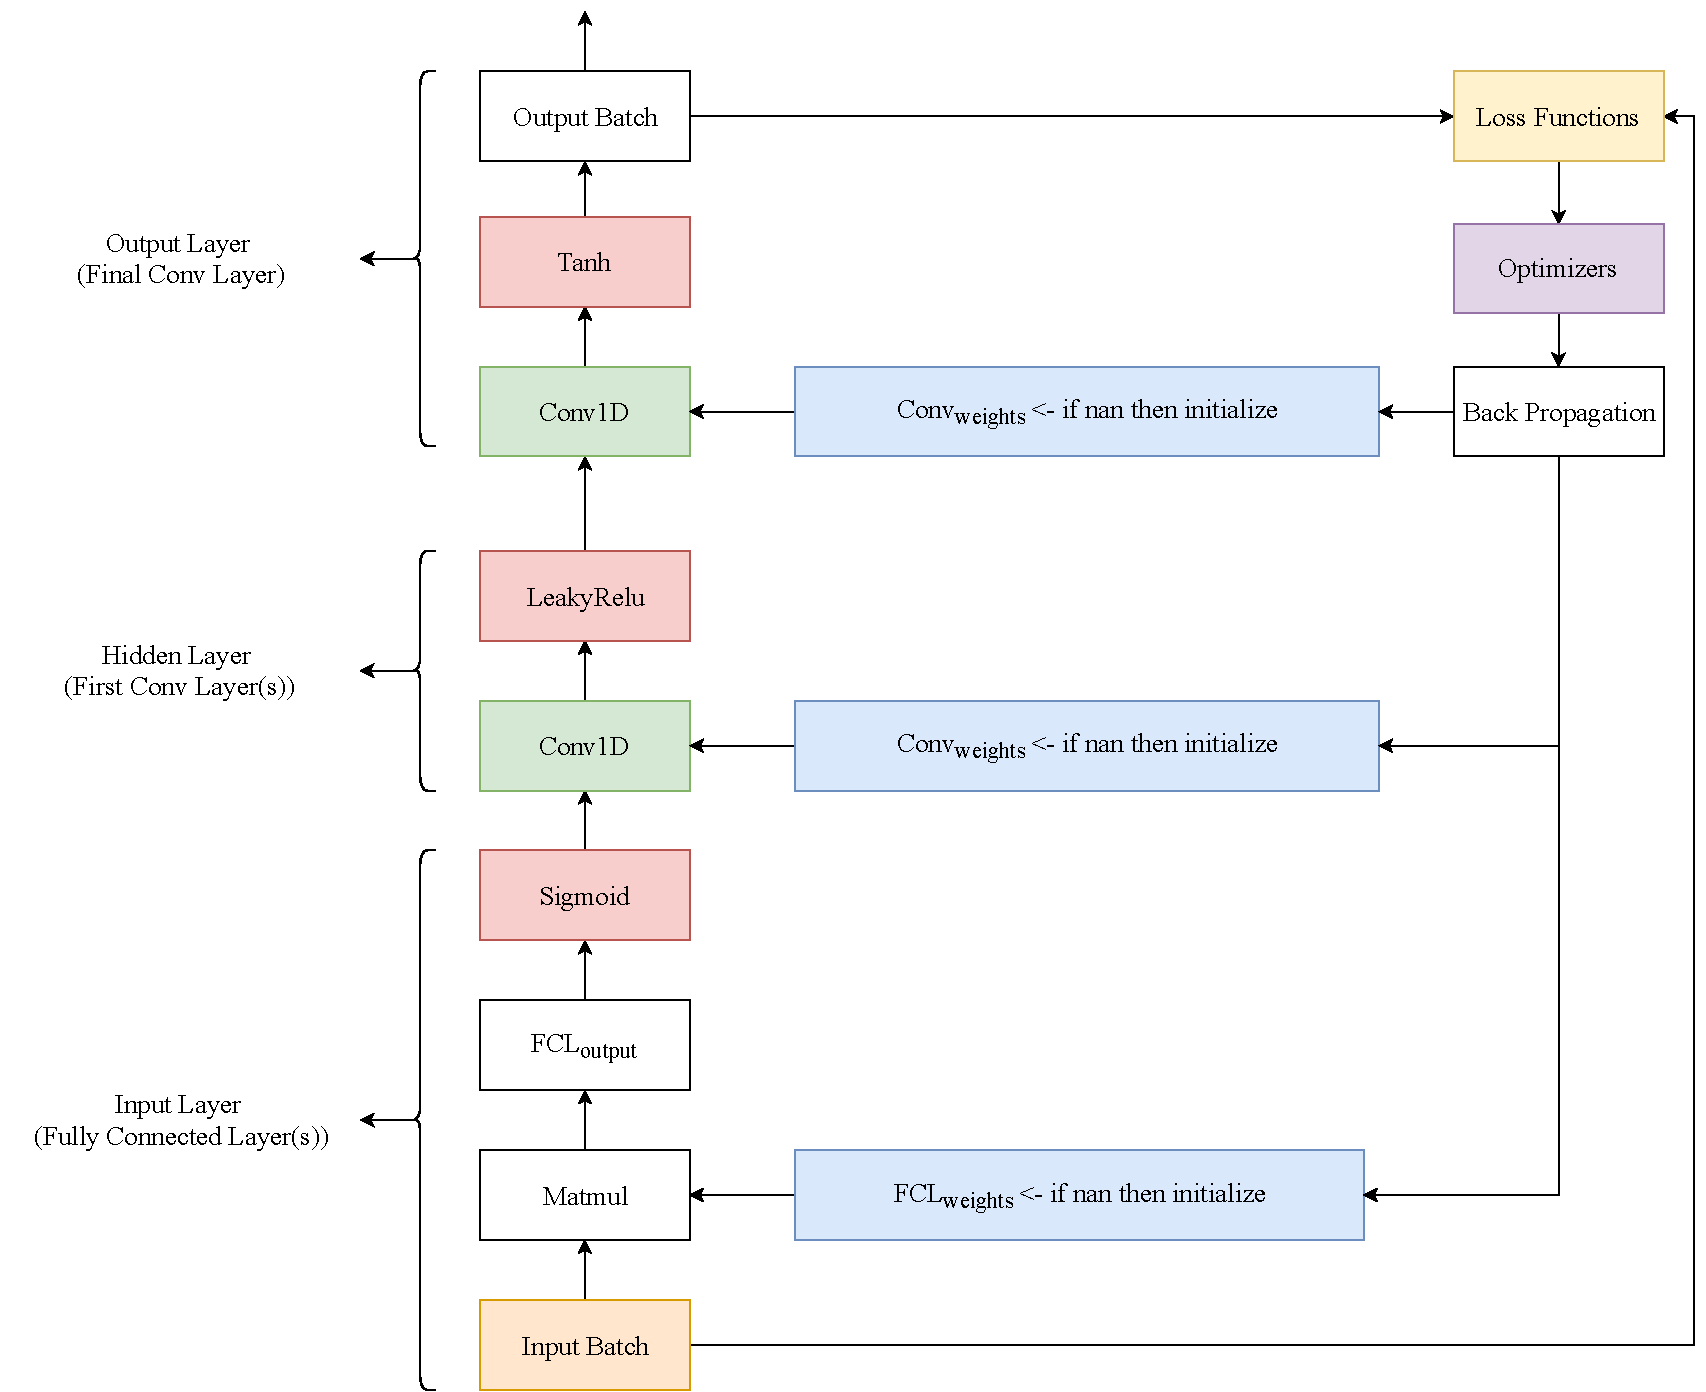
\includegraphics[height=0.9\textheight]{SimpleNetDiagram}
		\end{center}
	\end{frame}
		\begin{frame}{Activation Function Combinations}
			\textbf{Different Options:}
			\begin{itemize}
				\item $" Sigmoid \rightarrow LeakyRealu \rightarrow Sigmoid "$.
				\item $" Tanh \rightarrow LeakyRealu \rightarrow Tanh "$.
				\item $" Sigmoid \rightarrow LeakyRealu \rightarrow Tanh "$.
			\end{itemize}
			\textbf{The Empirically Reliable Choice:}\\
			\centering $" Sigmoid \rightarrow LeakyRealu \rightarrow Tanh "$.
		\end{frame}
		\begin{frame}{Activation Function Combinations - Numerical Analysis}
			$" Tanh \rightarrow LeakyRealu \rightarrow Tanh "$
			\begin{center}
				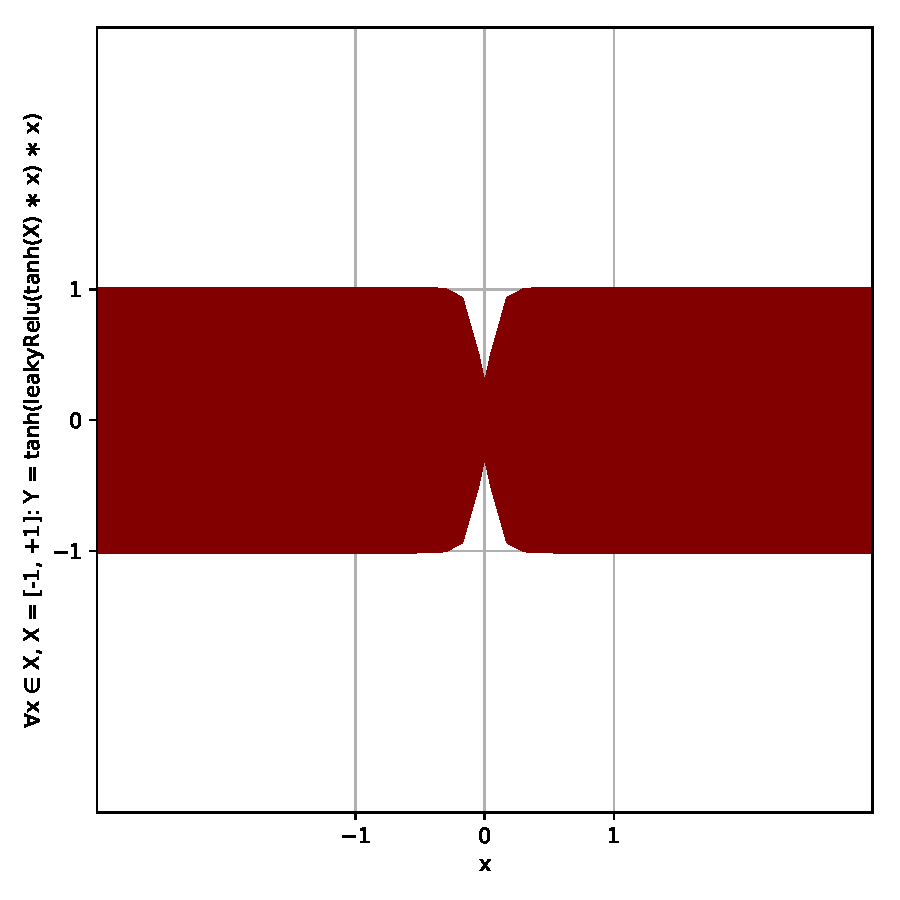
\includegraphics[height=0.9\textheight]{tanh_leakyRelu_tanh}
			\end{center}
		\end{frame}
		\begin{frame}{Activation Function Combinations - Numerical Analysis}
			$" Sigmoid \rightarrow LeakyRealu \rightarrow Sigmoid "$.
			\begin{center}
				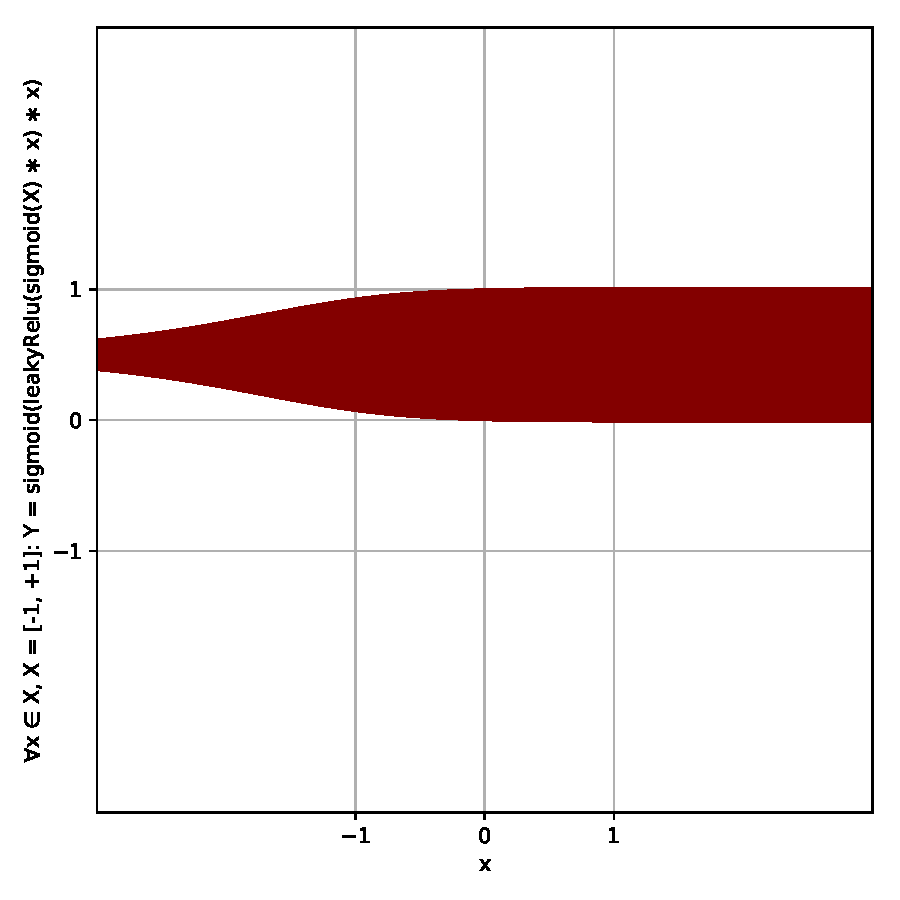
\includegraphics[height=0.9\textheight]{sigmoid_leakyRelu_sigmoid}
			\end{center}
		\end{frame}
		\begin{frame}{Activation Function Combinations - Numerical Analysis}
			$" Sigmoid \rightarrow LeakyRealu \rightarrow Tanh "$.
			\begin{center}
				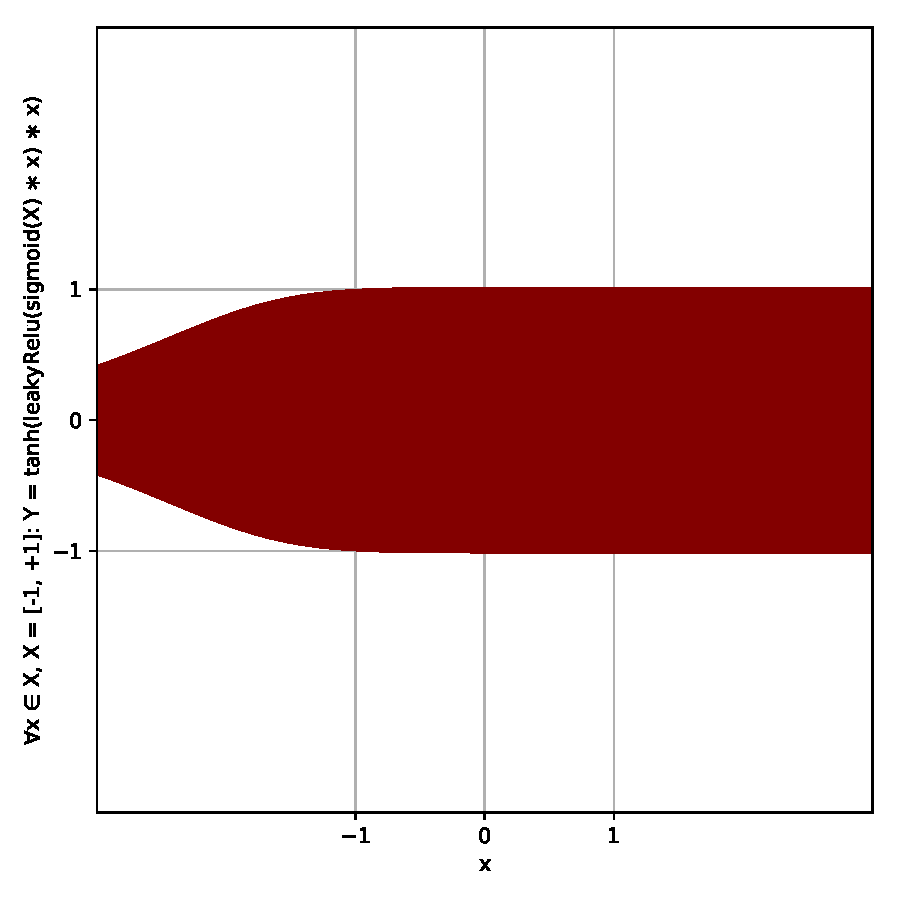
\includegraphics[height=0.9\textheight]{sigmoid_leakyRelu_tanh}
			\end{center}
		\end{frame}
		\begin{frame}
			\frametitle{References}
			\bibliographystyle{unsrt}
			\bibliography{../dissertation/latex_files/neurencoder.bib}
		\end{frame}
\end{document}
